\documentclass[journal,12pt,twocolumn]{IEEEtran}

\usepackage{setspace}
\usepackage{gensymb}
\singlespacing
\usepackage[cmex10]{amsmath}
\usepackage{amsthm}

\usepackage{mathrsfs}
\usepackage{txfonts}
\usepackage{stfloats}
\usepackage{bm}
\usepackage{cite}
\usepackage{cases}
\usepackage{subfig}

\usepackage{longtable}
\usepackage{multirow}
\usepackage{algorithm}
\usepackage{algorithmic}
\usepackage{enumitem}
\usepackage{mathtools}
\usepackage{steinmetz}
\usepackage{tikz}
\usepackage{circuitikz}
\usepackage{verbatim}
\usepackage{tfrupee}
\usepackage[breaklinks=true]{hyperref}
\usepackage{graphicx}
\usepackage{tkz-euclide}

\usetikzlibrary{calc,math}
\usepackage{listings}
    \usepackage{color}                                            %%
    \usepackage{array}                                            %%
    \usepackage{longtable}                                        %%
    \usepackage{calc}                                             %%
    \usepackage{multirow}                                         %%
    \usepackage{hhline}                                           %%
    \usepackage{ifthen}                                           %%
    \usepackage{lscape}     
\usepackage{multicol}
\usepackage{chngcntr}

\DeclareMathOperator*{\Res}{Res}

\renewcommand\thesection{\arabic{section}}
\renewcommand\thesubsection{\thesection.\arabic{subsection}}
\renewcommand\thesubsubsection{\thesubsection.\arabic{subsubsection}}

\renewcommand\thesectiondis{\arabic{section}}
\renewcommand\thesubsectiondis{\thesectiondis.\arabic{subsection}}
\renewcommand\thesubsubsectiondis{\thesubsectiondis.\arabic{subsubsection}}


\hyphenation{op-tical net-works semi-conduc-tor}
\def\inputGnumericTable{}                                 %%

\lstset{
%language=C,
frame=single, 
breaklines=true,
columns=fullflexible
}
\begin{document}


\newtheorem{theorem}{Theorem}[section]
\newtheorem{problem}{Problem}
\newtheorem{proposition}{Proposition}[section]
\newtheorem{lemma}{Lemma}[section]
\newtheorem{corollary}[theorem]{Corollary}
\newtheorem{example}{Example}[section]
\newtheorem{definition}[problem]{Definition}

\newcommand{\BEQA}{\begin{eqnarray}}
\newcommand{\EEQA}{\end{eqnarray}}
\newcommand{\define}{\stackrel{\triangle}{=}}
\bibliographystyle{IEEEtran}
\raggedbottom
\setlength{\parindent}{0pt}
\providecommand{\mbf}{\mathbf}
\providecommand{\pr}[1]{\ensuremath{\Pr\left(#1\right)}}
\providecommand{\qfunc}[1]{\ensuremath{Q\left(#1\right)}}
\providecommand{\sbrak}[1]{\ensuremath{{}\left[#1\right]}}
\providecommand{\lsbrak}[1]{\ensuremath{{}\left[#1\right.}}
\providecommand{\rsbrak}[1]{\ensuremath{{}\left.#1\right]}}
\providecommand{\brak}[1]{\ensuremath{\left(#1\right)}}
\providecommand{\lbrak}[1]{\ensuremath{\left(#1\right.}}
\providecommand{\rbrak}[1]{\ensuremath{\left.#1\right)}}
\providecommand{\cbrak}[1]{\ensuremath{\left\{#1\right\}}}
\providecommand{\lcbrak}[1]{\ensuremath{\left\{#1\right.}}
\providecommand{\rcbrak}[1]{\ensuremath{\left.#1\right\}}}
\theoremstyle{remark}
\newtheorem{rem}{Remark}
\newcommand{\sgn}{\mathop{\mathrm{sgn}}}
\providecommand{\abs}[1]{\left\vert#1\right\vert}
\providecommand{\res}[1]{\Res\displaylimits_{#1}} 
\providecommand{\norm}[1]{\left\lVert#1\right\rVert}
%\providecommand{\norm}[1]{\lVert#1\rVert}
\providecommand{\mtx}[1]{\mathbf{#1}}
\providecommand{\mean}[1]{E\left[ #1 \right]}
\providecommand{\fourier}{\overset{\mathcal{F}}{ \rightleftharpoons}}
%\providecommand{\hilbert}{\overset{\mathcal{H}}{ \rightleftharpoons}}
\providecommand{\system}{\overset{\mathcal{H}}{ \longleftrightarrow}}
	%\newcommand{\solution}[2]{\textbf{Solution:}{#1}}
\newcommand{\solution}{\noindent \textbf{Solution: }}
\newcommand{\cosec}{\,\text{cosec}\,}
\providecommand{\dec}[2]{\ensuremath{\overset{#1}{\underset{#2}{\gtrless}}}}
\newcommand{\myvec}[1]{\ensuremath{\begin{pmatrix}#1\end{pmatrix}}}
\newcommand{\mydet}[1]{\ensuremath{\begin{vmatrix}#1\end{vmatrix}}}
\numberwithin{equation}{subsection}
\makeatletter
\@addtoreset{figure}{problem}
\makeatother
\let\StandardTheFigure\thefigure
\let\vec\mathbf
\renewcommand{\thefigure}{\theproblem}
\def\putbox#1#2#3{\makebox[0in][l]{\makebox[#1][l]{}\raisebox{\baselineskip}[0in][0in]{\raisebox{#2}[0in][0in]{#3}}}}
     \def\rightbox#1{\makebox[0in][r]{#1}}
     \def\centbox#1{\makebox[0in]{#1}}
     \def\topbox#1{\raisebox{-\baselineskip}[0in][0in]{#1}}
     \def\midbox#1{\raisebox{-0.5\baselineskip}[0in][0in]{#1}}
\vspace{3cm}
\title{Assignment - FFT IMPLEMENTATION}
\author{BUEREDDY VARUNI - EE18BTECH11005}
\maketitle
\newpage
\bigskip
\renewcommand{\thefigure}{\theenumi}
\renewcommand{\thetable}{\theenumi}
Download all codes from 
\begin{lstlisting}
https://github.com/varunireddy/EE3025_IDP/tree/main/fft_implementation/codes
\end{lstlisting}
%
and latex-tikz codes from 
%
\begin{lstlisting}
https://github.com/varunireddy/EE3025_IDP/tree/main/fft_implementation
\end{lstlisting}
\section{Problem}
FFT implementation algorithm using recursive approach.
\section{Method - Recursive approach}
We compute DFT using the following equation.,
\begin{align}
    X(k) = \sum_{n=0}^{N-1}x[n]W_{N}^{kn} \label{eq:DFT_equation}\\
    \text{where.,} W_N = e^\frac{-2\pi i}{N}\\
    X(k) = \sum_{n=even}^{}x[n]W_{N}^{kn} + \sum_{n=odd}^{}x[n]W_{N}^{kn}
\end{align}
Let n = 2r in first term and n = 2r+1 in the second term.
\begin{align}
    X(k) &= \sum_{r=0}^{\frac{N}{2}-1}x[2r]W_{N}^{2kr} + \sum_{r=0}^{\frac{N}{2}-1}x[2r+1]W_{N}^{k(2r+1)} \label{eq:eq1}\\
\text{Let, }    x[2r]&=e[r] \text{, }x[2r+1]=o[r]\\
\end{align}
We know from the exponential property of complex numbers,
\begin{align}
    W_\frac{N}{2} = W_{N}^{2}
\end{align}
The equation.\ref{eq:eq1} can be rewritten as the following.,
\begin{align}
    X(k) &= \sum_{r=0}^{\frac{N}{2}-1}e[r]W_{N/2}^{kr} + W_{N}^k\sum_{r=0}^{\frac{N}{2}-1}o[r]W_{N/2}^{kr}
\end{align}
We can observe that the first term is the N/2 point DFT of even indices of the signal x[n] and the second term is the N/2 point DFT of odd indices of the signal x[n].
Therefore, the equation $\forall$ k in [0,N/2) can be written as, 
\begin{align}
    X(k) &= E(k) + W_{N}^k O(k)  \label{eq:eq2}
\end{align}
Where E(k) is the dft of the even indices and O(k) is the dft of the odd indices of x[n].
For $\forall$ k+N/2 in [N/2,N) the equation can be written as,
\begin{align}
    X(k+N/2) &= E(k+N/2) + W_{N}^{k+N/2} O(k+N/2)\\
    X(k+N/2) &= E(k) - W_N^k O(k) \label{eq:eq3}
\end{align}
If $F_N$ is the N point DFT matrix and $F_{N/2}$ is the N/2 point DFT matrix.
\begin{align}
    X(k) &= F_N x[n]\\
    E(k) &= F_{N/2} e[n]\\
    O(k) &= F_{N/2} o[n]
\end{align}
From the equations.\ref{eq:eq2} and \ref{eq:eq3},\\ for k in [0,N/2)..,
\begin{align}
    F_N x[n] = F_{N/2} e[n] +F_{N/2}D_{N/2} o[n]
\end{align}
for k in [N/2,N)..,
\begin{align}
    F_N x[n] = F_{N/2} e[n] -F_{N/2}D_{N/2} o[n]
\end{align}
where $D_N$ is the diagonal matrix with diagonal values $[1,W_N^1,W_N^2,W_N^3...,W_N^{N-1}]$.\\
Combining the above two equations, 
\begin{align}
    F_N x[n] = \begin{bmatrix}I_{N/2} & D_{N/2} \\ I_{N/2} & -D_{N/2} 
    \end{bmatrix} \begin{bmatrix}F_{N/2} & 0 \\ 0 & F_{N/2} 
    \end{bmatrix} \begin{bmatrix}e[n]\\ o[n] \label{eq:eq4}
    \end{bmatrix}
\end{align}
Let P be the transformation matrix., which transforms x[n] into [e[n] o[n]].
\begin{align}
    \begin{bmatrix}e[n]\\ o[n] 
    \end{bmatrix} = [P]_{N\times N}x[n] \label{eq:eq5}
\end{align}
where.,
\begin{align}
     P = \begin{bmatrix}1 & 0 & 0 & 0 &\hdots{} & 0\\
    0 & 0 & 1 & 0 & \hdots{} & 0\\ \vdots{} \\ 0 & 1 & 0 & 0 & \hdots{} & 0\\
    0 & 0 & 0 & 1 &\hdots{} & 0\\ \vdots{} \\
    0 & 0 & 0&0 &\hdots{} & 1
    \end{bmatrix}
\end{align}
From equations.\ref{eq:eq4} and \ref{eq:eq5} we get.,
\begin{align}
     F_N = \begin{bmatrix}I_{N/2} & D_{N/2} \\ I_{N/2} & -D_{N/2} 
    \end{bmatrix} \begin{bmatrix}F_{N/2} & 0 \\ 0 & F_{N/2} 
    \end{bmatrix}P 
\end{align}
Thus, we can now compute $F_N$ from $F_{N/2}$, $F_{N/2}$ from $F_{N/4}$. This is the recursive approach. N=1 is the base case. 
When N = 1, FFT(x) = x.
\begin{figure}[!ht]
    \centering
    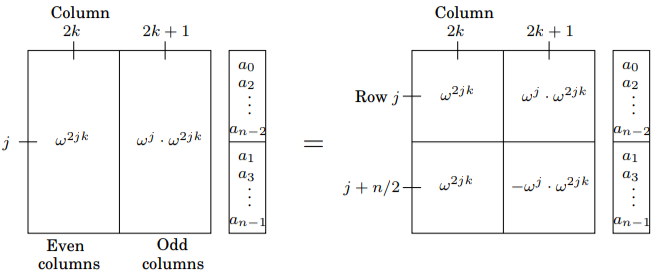
\includegraphics[width=9cm]{./figs/subblock.png}
    \caption{Recursive sub block approach}
    \label{fig:fig1}
\end{figure}
\section{Pseudo Code}
\begin{algorithm}
\caption{fft(x)}
\begin{algorithmic} 
\REQUIRE $N > 0$
\ENSURE $N = 2^n$
\STATE N $\leftarrow$ length(x)
\IF{$N = 1$}
\STATE Return x
\ELSE
\STATE E $\leftarrow$ fft(x[0],x[2]...,x[N-2])
\STATE O $\leftarrow$ fft(x[1],x[3]...,x[N-1])
\WHILE{$k \neq N/2-1$}
\STATE X[k] $\leftarrow$ E[k] + $e^{2\pi jk/N}$ O[k]
\STATE X[k+N/2] $\leftarrow$ E[k] - $e^{2\pi jk/N}$ O[k]
\ENDWHILE
\STATE Return X
\ENDIF
\end{algorithmic}
\end{algorithm}

%---------------------------
\section{FFT Implementation in Python}

 Let x[n] = \cbrak{\underset{\uparrow}{1},2,3,4,4,3,2,1}\\
$N = 8 = 2^3$. We need to compute the 8-point DFT using the above mentioned recursive algorithm in Python. 

\begin{align}
    X &= F_8 x[n]\\
    F_8 &= \begin{bmatrix}I_4 & D_4\\I_4 & -D_4  \end{bmatrix} \begin{bmatrix} F_4 & 0 \\0 & F_4
    \end{bmatrix}P_8\\
    D_4 &= diag[0,W_4^1,W_4^2,W_4^3]\\
    P_8 &= \begin{bmatrix}
    1 & 0 & 0 & 0 & 0 & 0 & 0 & 0\\
    0 & 0 & 1 & 0 & 0 & 0 & 0 & 0\\
    0 & 0 & 0 & 0 & 1 & 0 & 0 & 0\\
    0 & 0 & 0 & 0 & 0 & 0 & 1 & 0\\
    0 & 1 & 0 & 0 & 0 & 0 & 0 & 0\\
    0 & 0 & 0 & 1 & 0 & 0 & 0 & 0\\
    0 & 0 & 0 & 0 & 0 & 1 & 0 & 0\\
    0 & 0 & 0 & 0 & 0 & 0 & 0 & 1\\
    \end{bmatrix}
\end{align}
Our goal is to compute X, for which we need to find $F_8$, which can be computed from $F_4$. 
\begin{align}
    F_4 &= \begin{bmatrix}I_2 & D_2\\I_2 & -D_2  \end{bmatrix} \begin{bmatrix} F_2 & 0 \\0 & F_2
    \end{bmatrix}P_4\\
     F_2 &= \begin{bmatrix}1 & D_1\\1 & -D_1  \end{bmatrix} \begin{bmatrix} F_1 & 0 \\0 & F_1
    \end{bmatrix}P_2\\
    F_1 &= 1
\end{align}
Thus, we recursively compute 8 point DFT from two 4 point DFT's and 4 point DFT's from two 2 point DFT's. The following python code is the implementation of the above algorithm. 
\begin{lstlisting}
https://github.com/varunireddy/EE3025_IDP/blob/main/fft_implementation/codes/ee18btech11005.py
\end{lstlisting}
\begin{figure}
    \centering
    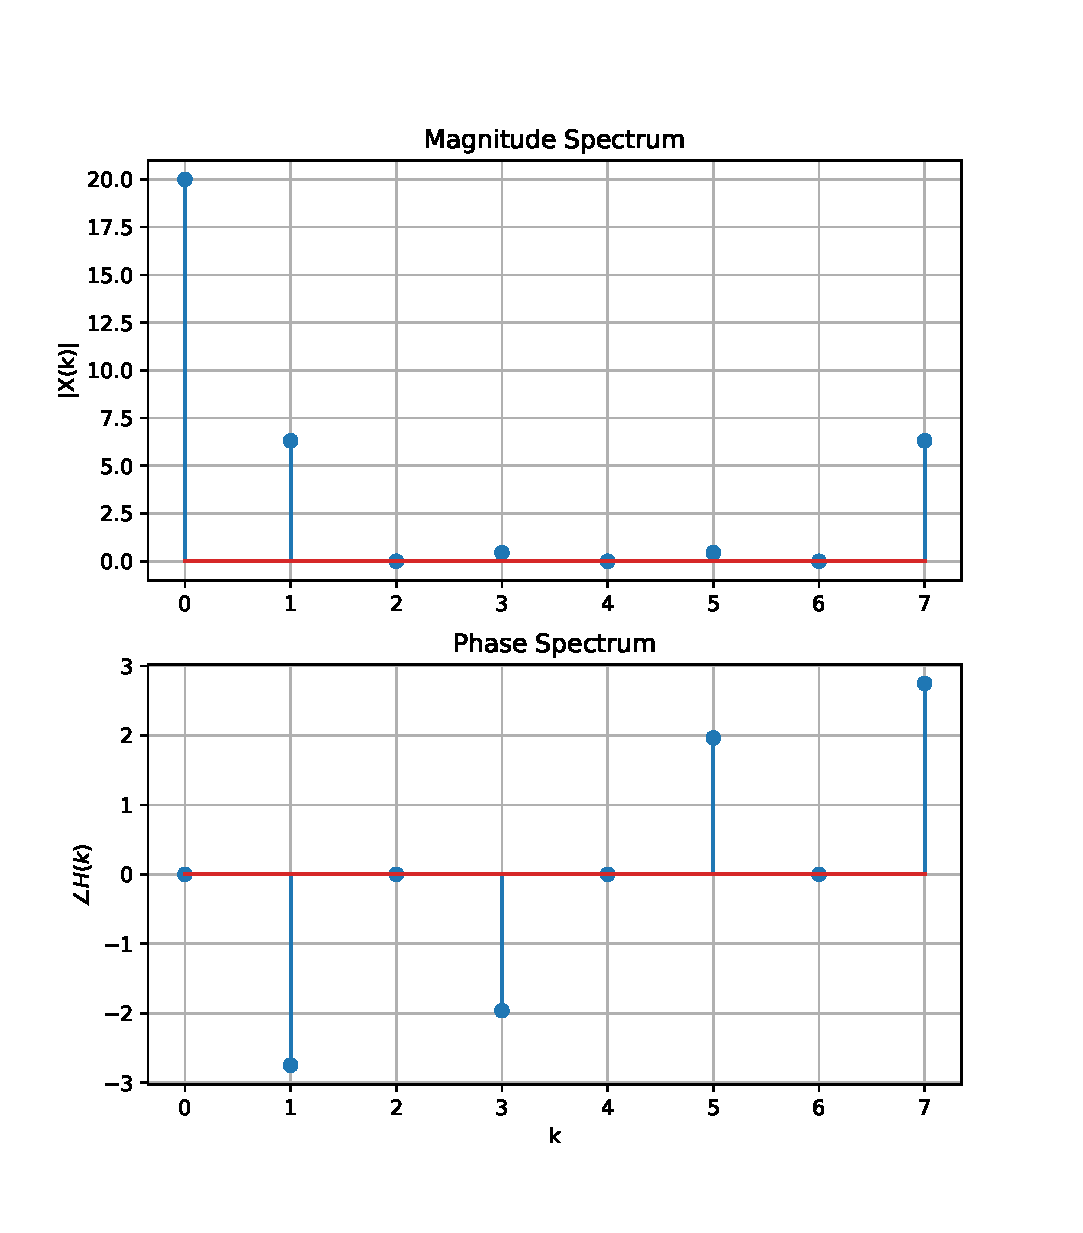
\includegraphics[width=9cm]{./figs/fft_py.eps}
    \caption{FFT implementation in python}
    \label{fig:fft_py}
\end{figure}
The above code generates the Figure.\ref{fig:fft_py} FFT implementation in python.

\section{FFT Implementation in C}
We can use the divide and conquer approach in C. The following C code generates the .dat binary file which contains the real and imaginary parts of the fft.\\
\begin{lstlisting}
https://github.com/varunireddy/EE3025_IDP/blob/main/fft_implementation/codes/ee18btech11005.c
\end{lstlisting}
The following python code generates the plots from the .dat file generated by running the above C code
\begin{lstlisting}
https://github.com/varunireddy/EE3025_IDP/blob/main/fft_implementation/codes/read_dat_file.py
\end{lstlisting}
\begin{figure}[!ht]
    \centering
    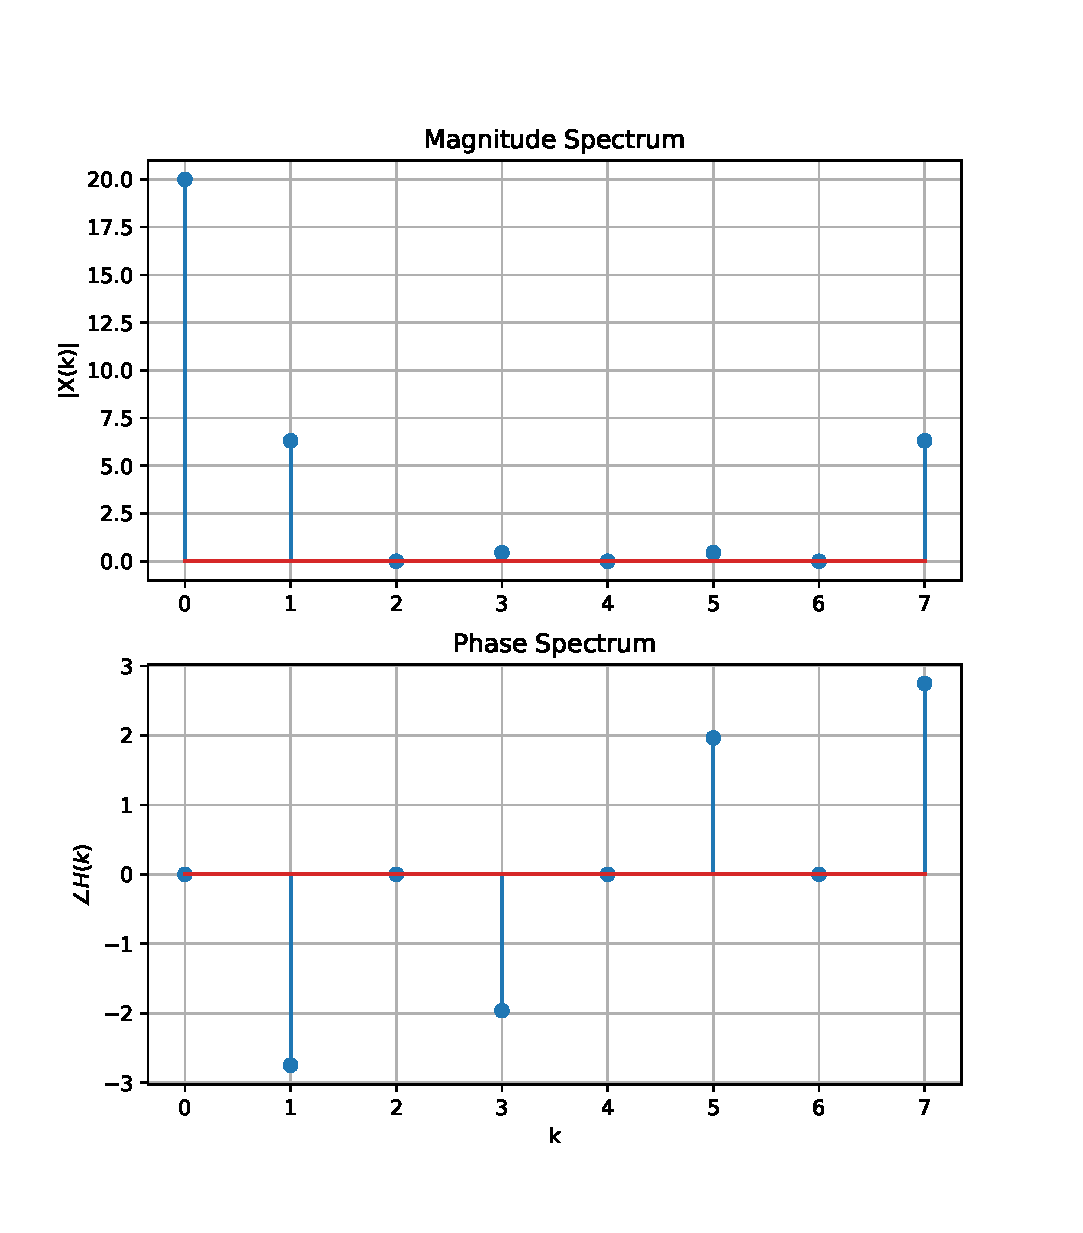
\includegraphics[width=9cm]{./figs/fft_c.eps}
    \caption{FFT implementation in C}
    \label{fig:fft_c}
\end{figure}
Figure.\ref{fig:fft_c} is the implementation of the fft algorithm in C and plotting the spectrum in python.
\section{Time Complexity}
The traditional DFT algorithm has two nested for loops, So the time complexity is O($N^2$).
But we can notice that the FFT algorithm with N inputs has $\log_2 N$ levels, each with N nodes, for a total of N$\log_2 N$ operations that is one N point FFT can be broken down into two N/2 point fft's. 
\begin{align}
    T(n) = 2T(n/2) + O(n)
\end{align}
Thus, the time complexity of the FFT algorithm using recursive subblock approach is O(N$\log_2 N$) whereas for a DFT algorithm time complexity is O($N^2$).\\
The following code compares the computation times for a DFT algorithm and FFT algorithm.
\begin{lstlisting}
https://github.com/varunireddy/EE3025_IDP/blob/main/fft_implementation/codes/comparetime.py
\end{lstlisting}

\begin{figure}[!ht]
    \centering
    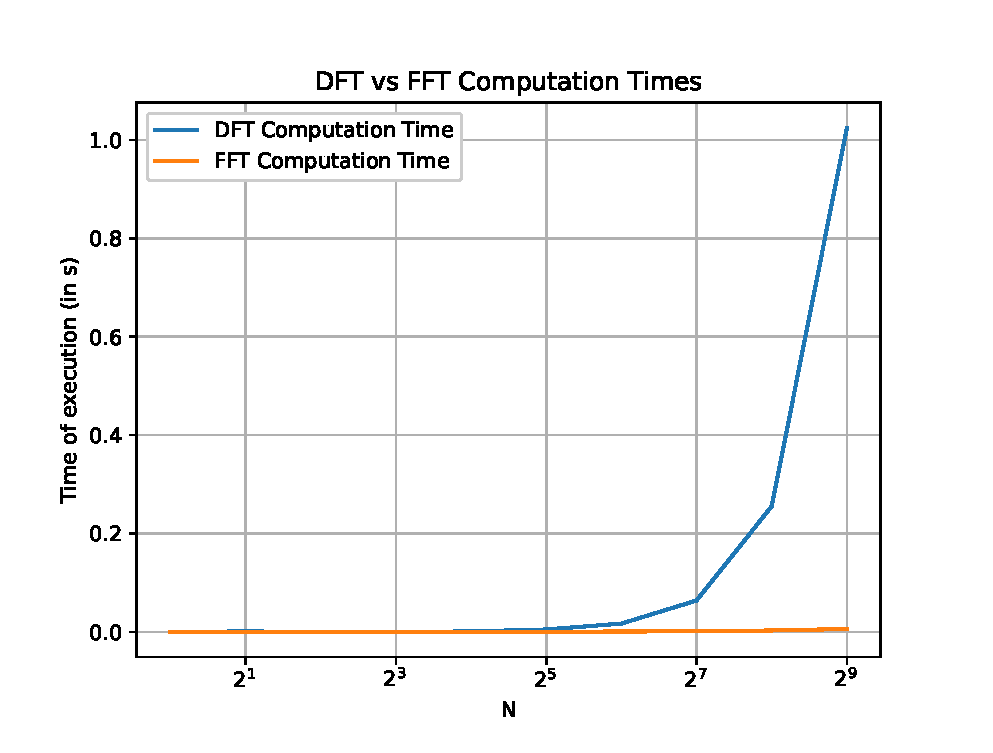
\includegraphics[width=9cm]{./figs/comparetime.eps}
    \caption{DFT vs FFT}
    \label{fig:comparison}
\end{figure}
\section{Conclusions}
The Fast Fourier Transform (FFT) is an implementation of the DFT which produces almost the same results as the DFT, but it is incredibly more efficient and much faster which often reduces the computation time significantly. Therefore, FFT is a computational algorithm used for fast and efficient computation of the DFT.
\end{document}